\documentclass[conference]{IEEEtran}
\usepackage{amsmath,amssymb,booktabs,graphicx,array,multirow,url}
\usepackage[T1]{fontenc}
\usepackage{lmodern}
\usepackage{microtype}
\usepackage[hidelinks]{hyperref}
\newcommand{\ind}{\mathbf{1}}
\newcommand{\R}{\mathbb{R}}
\title{When AI Exposure Rankings Disagree: Robust Top-25 Selection Across 661 U.S. Occupations}
\author{\IEEEauthorblockN{Ghassan Malkawi$^{1}$, Ahmed Abdelaziz Elsayed$^{2}$, Asem Omari$^{1}$,\\Azmi Alazzam$^{1}$, Said Badreddine$^{1}$, Shaima Alharthi$^{1}$}
\IEEEauthorblockA{$^{1}$Faculty of Computer Information Science, Higher Colleges of Technology\\Al Ain, Abu Dhabi, United Arab Emirates\\
\{gmalkawi,aomari,aalazzam,sbadreddine\}@hct.ac.ae; H00543372@hct.ac.ae}
\IEEEauthorblockA{$^{2}$Department of Computer Engineering and Computational Sciences, Canadian University Dubai\\Dubai, United Arab Emirates\\
ahmed.elsayed@cud.ac.ae}}
\begin{document}
\maketitle
\begin{abstract}
AI-exposure measures do not necessarily identify the same occupations as priorities. This creates a practical problem when institutions must choose a fixed set of occupations for workforce screening and further occupational assessment. Using 661 U.S. occupations and 18 coherent AI-exposure specifications, we ask which occupations remain stable priorities and which fixed Top-25 list is least sensitive to the admitted measurement-design family. Under coherent designs, 14 occupations appear in every Top-25 and 37 appear in at least one; the more conservative independent interval box gives only 4 guaranteed and 87 possible members. A relative-minimax list raises worst-scenario capture from 93.70\% for the baseline composite to 96.52\%, although its exact independent-box absolute regret is slightly larger (0.01945 versus 0.01810). We derive exact best/worst rank certificates, a lossless existence-based screening theorem, and an exact fixed-list box-regret corner formula. A nested-support sensitivity then shows where membership conclusions change as the box contracts toward a declared point core. The reported values $g^\star=0.574320$, $0.434651$, and $0.078756$ are transition boundaries: because best rank uses a strict comparison and worst rank a non-strict comparison, post-contraction membership applies immediately below the relevant boundary rather than being asserted at equality. The resulting Top-25 is a screening and further-assessment list, not a displacement forecast, transition probability, or program-success prediction.
\end{abstract}
\begin{IEEEkeywords}
AI exposure, occupational prioritization, robust Top-$k$, uncertain ranking, minimax regret, workforce screening
\end{IEEEkeywords}

\section{Results First: What Changes for Workforce Screening?}
Occupational AI-exposure rankings can vary materially with measurement design, so a single printed ranking can conceal decision instability \cite{yin2026}. At $k=25$, only 14 of 661 occupations occur in every coherent Top-25 list, while 37 occur in at least one. The independent coordinatewise interval box is intentionally more conservative: it certifies only 4 guaranteed members and 87 possible members. Table~\ref{tab:stability} converts those counts into a direct screening interpretation.

\begin{table}[t]
\caption{Occupational stability under coherent AI-exposure disagreement at $k=25$.}
\label{tab:stability}
\centering\small
\begin{tabular}{p{0.29\columnwidth}p{0.48\columnwidth}r}
\toprule
Status & Interpretation & $n$\\
\midrule
Stable & In every coherent Top-25 & 14\\
Design-sensitive & In some but not all coherent Top-25 lists & 23\\
Outside family & In no coherent Top-25 list & 624\\
\bottomrule
\end{tabular}
\end{table}

The stable set spans managerial, professional, service, sales, clerical, transportation, and logistics occupations. Examples include General and Operations Managers, Accountants and Auditors, Registered Nurses, Cashiers, Retail Salespersons, Office Clerks, Heavy and Tractor-Trailer Truck Drivers, and Stockers and Order Fillers; the full 14-occupation set with SOC codes is reported in the Supplement.

When one fixed list is required, the relative-minimax solution retains at least 96.52\% of each scenario's own optimal Top-25 priority mass. The baseline composite retains at least 93.70\%. Thus the applied question is not ``which ranking is true?'' but ``which priorities are stable across admitted designs, and what fixed list limits worst-case loss when designs disagree?'' The mathematics below supplies exact certificates for that decision.

\begin{figure}[t]
\centering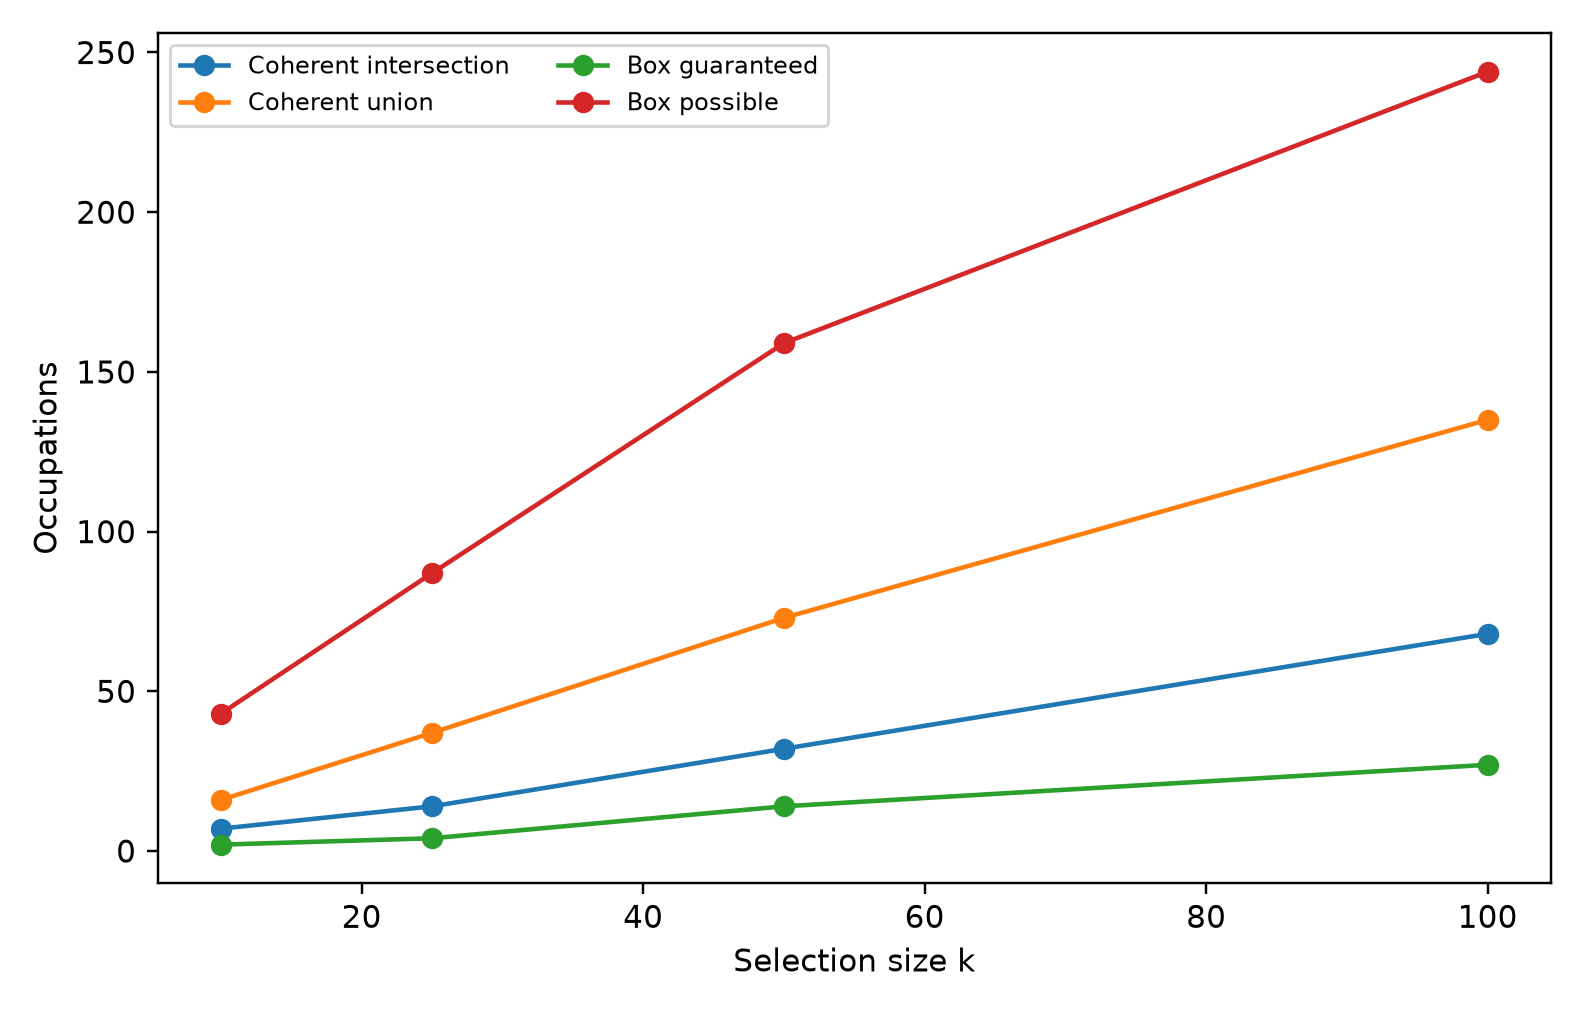
\includegraphics[width=\columnwidth]{figures/membership.png}
\caption{Membership envelopes across evaluated selection sizes. Coherent specifications move occupational scores together, whereas the independent box permits coordinatewise adversarial movement.}
\label{fig:membership}
\end{figure}

\section{Decision Problem and Coherent Uncertainty}
Let $i\in\{1,\ldots,n\}$ index occupations. The application uses AI Occupational Exposure (AIOE) as one exposure channel \cite{felten2021} and two Microsoft applicability channels (user-goal and AI-action/nonphysical) \cite{tomlinson2025}. Scale $s_i$ is May 2025 OEWS employment share \cite{bls2026}, and the five occupation-level skill descriptors are from O*NET 30.3 \cite{onet2026}.

To make the modifier construction explicit, let $a_i^{(r)}\in[0,1]$ be the frozen normalized exposure value for channel $r$, and let $z_{im}\in[0,1]$ be the frozen normalized O*NET Importance value for skill $m$ in occupation $i$. The five skills are Critical Thinking, Active Learning, Learning Strategies, Active Listening, and Speaking. For construction $w$ with retained skill set $M_w$, define
\begin{equation}
h_i^{(w)}=\frac{1}{|M_w|}\sum_{m\in M_w}z_{im},
\label{eq:hac}
\end{equation}
where the equal-five construction uses all five skills and each of the five ablations removes exactly one skill. The exposure-conditioned modifier and employment-scaled priority are
\begin{equation}
q_i^{(r,w)}=a_i^{(r)}\bigl(1-h_i^{(w)}\bigr),\qquad
p_i^t=s_iq_i^{(r,w)},
\label{eq:priority}
\end{equation}
with $t=(r,w)$. The factor $1-h_i^{(w)}$ is a declared screening transformation: a larger retained-skill aggregate lowers the modifier within this construction, but it is not causal evidence that skills protect a worker from AI exposure or displacement. The paper treats the normalized exposure and skill inputs as frozen primitive inputs to the decision layer; it does not re-estimate their upstream measurement models. This construction follows transparent composite-indicator and multiverse practice: admitted designs are kept coherent rather than replaced by arbitrary coordinatewise combinations \cite{oecd2008,manski2003,greco2008,steegen2016,simonsohn2020}.

The application fixes $n=661$ U.S. occupations and $T=18$ primitive scenarios: three exposure channels times six skill constructions. For each occupation,
\begin{equation}
\ell_i=\min_t p_i^t,\qquad u_i=\max_t p_i^t,
\label{eq:bounds}
\end{equation}
and
\begin{equation}
\mathcal P_{\square}=\prod_{i=1}^n[\ell_i,u_i],\qquad
\mathcal P_T=\{p^t:t=1,\ldots,T\}\subseteq\mathcal P_{\square}.
\end{equation}
The declared point core $c_i=p_i^{\mathrm{AIOE,equal-five}}$ is one primitive scenario, hence
\begin{equation}
\ell_i\le c_i\le u_i\qquad \forall i.
\label{eq:coreinside}
\end{equation}
No probability distribution is assigned to either uncertainty set.

\section{Exact Independent-Box Rank Certificates}
Uncertain-ranking research distinguishes items that can attain a rank from items that must remain inside a rank range \cite{soliman2009,mouratidis2015,mouratidis2018}. Here tie treatment is asymmetric by construction. Best rank is existential and resolves endpoint ties in occupation $i$'s favor; worst rank is pessimistic and counts ties against $i$:
\begin{align}
r_i^{\min}&=1+\sum_{j\ne i}\ind\{\ell_j>u_i\},\\
r_i^{\max}&=1+\sum_{j\ne i}\ind\{u_j\ge\ell_i\}.
\label{eq:ranks}
\end{align}
Here $\ind\{\cdot\}$ denotes the indicator function. The endpoint realizations are feasible in $\mathcal P_{\square}$, so the certificates are exact:
\begin{align}
i\text{ guaranteed Top-}k&\iff r_i^{\max}\le k,\\
i\text{ possible Top-}k&\iff r_i^{\min}\le k.
\end{align}
Figure~\ref{fig:membership} shows how the box and coherent envelopes differ over $k\in\{10,25,50,100\}$.

\section{Coherent Fixed-List Relative Minimax}
The fixed-list decision is a finite minimax-regret selection problem over the declared coherent scenarios \cite{bertsimas2003,bertsimas2004,bertsimas2011,aissi2009,ide2016,roy2010}. Let $V_k(p)$ be the sum of the $k$ largest components of $p$, and define $V_t^\star=V_k(p^t)$. For all admitted scenarios, $V_t^\star>0$. For binary selection $x_i\in\{0,1\}$ with $\sum_i x_i=k$, coherent capture and relative regret are
\begin{equation}
C_t(x)=\frac{\sum_i p_i^t x_i}{V_t^\star},\qquad R_t(x)=1-C_t(x).
\end{equation}
The fixed-list problem is
\begin{align}
\min_{x,\rho}\quad &\rho\\
\text{s.t.}\quad &\sum_i p_i^t x_i\ge(1-\rho)V_t^\star,\quad \forall t,\\
&\sum_i x_i=k,\quad x_i\in\{0,1\},\quad 0\le\rho\le1.
\label{eq:minimax}
\end{align}
Relative-regret and uncertain-return selection formulations provide the closest optimization context \cite{averbakh2005,kouvelis1997,savage1951,conde2004,kasperski2008}. Here $\rho$ is a worst relative shortfall, not a probability.

\subsection{Lossless screening}
Let $G=\{i:r_i^{\max}\le k\}$ and $Z=\{i:r_i^{\min}>k\}$.

\textit{Theorem 1 (existence-based lossless screening).} Assume $\mathcal P_T\subseteq\mathcal P_{\square}$. For any minimization objective $F(M_1(x),\ldots,M_T(x))$ that is coordinatewise nonincreasing in scenario-wise selected masses $M_t(x)=\sum_i p_i^t x_i$, there exists an optimum containing every item in $G$ and no item in $Z$.

\textit{Proof sketch.} Order the items of $G$ by nonincreasing lower bound and insert them in that order. If the next $a\in G$ is absent from a size-$k$ optimum, then at most $k-1$ competitors satisfy $u_j\ge\ell_a$, so the list contains some $h$ with $u_h<\ell_a$. Any guaranteed item $a'$ inserted earlier satisfies $\ell_{a'}\ge\ell_a$ and therefore $u_{a'}\ge\ell_{a'}\ge\ell_a$, so it cannot be this $h$. Replacing $h$ by $a$ thus preserves all earlier insertions and weakly increases every scenario-wise selected mass. After all $G$ items are inserted, if a selected $i\in Z$ remains, at least $k$ competitors satisfy $\ell_j>u_i$, so some omitted $j$ strictly dominates $i$ in every scenario. Replacing $i$ by $j$ strictly increases every scenario-wise selected mass. Because the family of size-$k$ lists is finite, strict exchanges cannot cycle. The process therefore terminates at an optimum containing all $G$ and no $Z$. $\square$

At $k=25$ the screening rule fixes 4 occupations as included and excludes 574 occupations as impossible members without changing the coherent optimum.

\section{Exact Independent-Box Regret of a Fixed List}
For a fixed set $X=\{i:x_i=1\}$, $|X|=k$, define absolute box regret
\begin{equation}
R_{\square}^{\mathrm{abs}}(X)=\max_{p\in\mathcal P_{\square}}\left[V_k(p)-\sum_{i\in X}p_i\right].
\end{equation}
The maximizing corner is
\begin{equation}
v_i(X)=\begin{cases}\ell_i,&i\in X,\\u_i,&i\notin X,\end{cases}
\end{equation}
so the exact closed form is
\begin{equation}
R_{\square}^{\mathrm{abs}}(X)=V_k(v(X))-\sum_{i\in X}\ell_i.
\label{eq:boxregret}
\end{equation}
Writing the expression with $V_k$ avoids ambiguity over the identity of a tied Top-$k$ corner set.

\section{Nested-Support Contraction and Exact Boundaries}
Possibilistic and interval-weight approaches can parameterize uncertain decision inputs \cite{kasperski2010,dubois2016}. Possibility theory is used only as optional parameterization language: the empirical object is a finite priority support plus a declared point core, not a calibrated possibility distribution. Retained support width $g\in[0,1]$ defines
\begin{equation}
L_i(g)=c_i-g(c_i-\ell_i),\qquad U_i(g)=c_i+g(u_i-c_i).
\label{eq:contract}
\end{equation}
By~\eqref{eq:coreinside}, this is a nested family with $g=1$ equal to the full box and $g=0$ equal to the point core.

Rank vectors are piecewise constant. We denote each reported structural transition boundary by $g^\star$. A best-rank comparison changes only at $L_j(g)=U_i(g)$,
\begin{equation}
g_{ji}^{(B)}=\frac{c_j-c_i}{(c_j-\ell_j)+(u_i-c_i)},
\end{equation}
and a worst-rank comparison only at $U_j(g)=L_i(g)$,
\begin{equation}
g_{ji}^{(W)}=\frac{c_i-c_j}{(u_j-c_j)+(c_i-\ell_i)},
\end{equation}
when the denominator is positive and the ratio lies in $[0,1]$. Thus all events follow from a finite exact breakpoint set rather than Monte Carlo sampling.

\begin{table}[t]
\caption{Reported Top-25 structural contraction boundaries.}
\label{tab:break}
\centering\small
\resizebox{\columnwidth}{!}{%
\begin{tabular}{lccc}
\toprule
Event & $g^\star$ & $1-g^\star$ & Interpretation\\
\midrule
Guaranteed $\to14$ & .574320 & .425680 & coherent intersection\\
Possible $\to37$ & .434651 & .565349 & cardinality; 32 shared\\
Full 25/25 & .078756 & .921244 & point list\\
\bottomrule
\end{tabular}}
\end{table}

The endpoint convention matters. Since best rank uses $L_j>U_i$ while worst rank uses $U_j\ge L_i$, $g^\star$ is a \emph{transition boundary}. When contraction proceeds from $g=1$ toward zero, the post-contraction membership state applies for $g<g^\star$; a newly strict best-rank comparison is not asserted at equality. Table~\ref{tab:break} therefore reports boundaries rather than ``first-at-equality'' events.

For any strictly decreasing homeomorphism $\phi:[0,1]\to[0,1]$ with $\phi(0)=1$ and $\phi(1)=0$, setting $g=\phi(\alpha)$ traverses the same nested supports in the same order. Examples $\phi(\alpha)=1-\alpha$ and $\phi(\alpha)=(1-\alpha)^2$ change numerical $\alpha$ labels but not the structural event sequence.

\begin{figure}[t]
\centering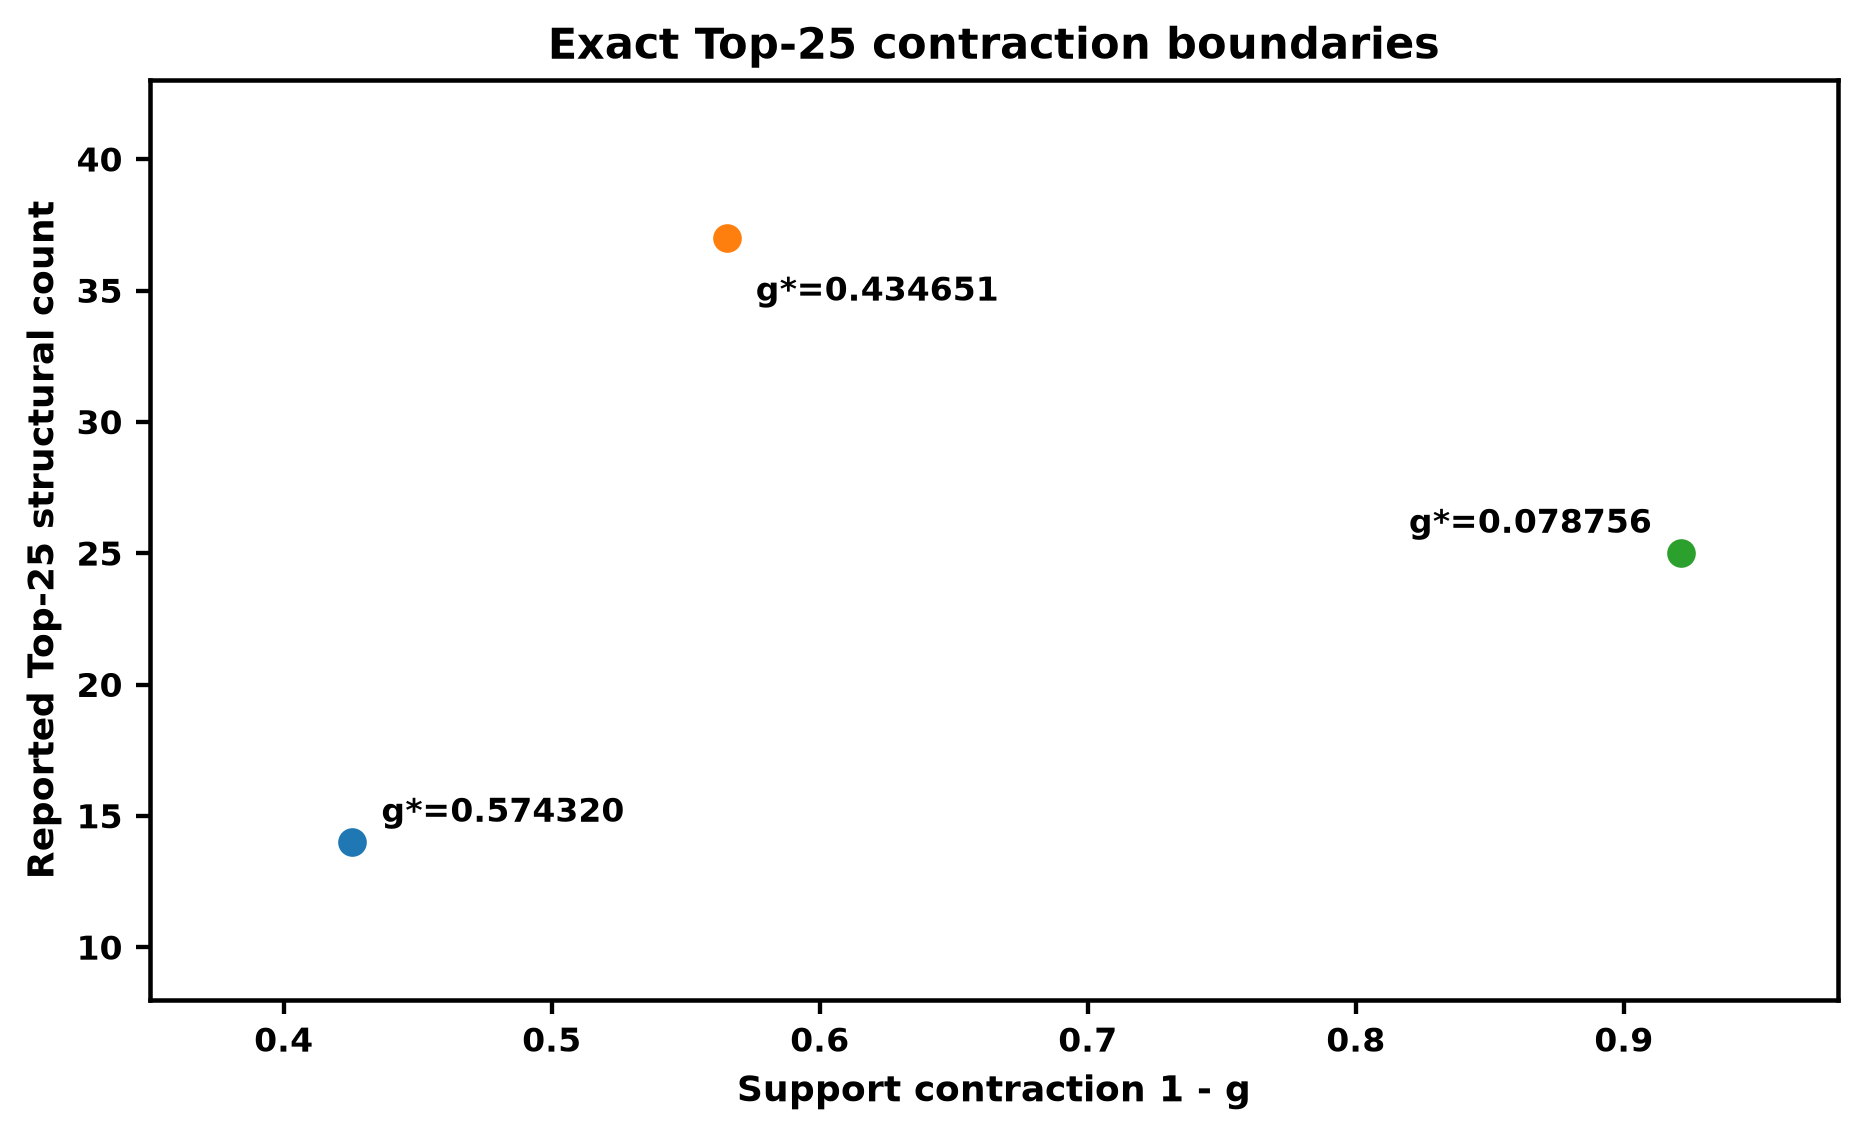
\includegraphics[width=\columnwidth]{figures/contraction_events.png}
\caption{Three reported exact Top-25 contraction boundaries. Points mark structural transition values; post-contraction membership follows the stated tie convention.}
\label{fig:contract}
\end{figure}

\section{Application Results}
Table~\ref{tab:performance} compares the three primary fixed-list rules and one transparent consensus benchmark. The relative-minimax list improves the minimum coherent-scenario capture to 96.52\%, from 93.70\% for the baseline composite and 88.35\% for scale only. Its exact box absolute regret is 0.01945, slightly larger than the baseline's 0.01810, so no list is unconditionally ``most robust'' without naming the uncertainty structure and criterion.

As a descriptive rank-aggregation benchmark, let $T_t=\operatorname{Top}_{25}(p^t)$ denote the set of the 25 occupations with the largest priorities under scenario $t$, and define
\begin{equation}
f_i=\sum_{t=1}^{18}\ind\{i\in T_t\}.
\label{eq:consensus}
\end{equation}
The Consensus-Frequency list contains the 25 occupations with the largest $f_i$. The 25th-ranked count is 9 and the 26th-ranked count is 8, so no frequency tie occurs at the membership cutoff; ascending SOC is retained only as a fixed deterministic tie-break for equal counts away from the cutoff. Because the 18 scenarios are declared designs rather than probability-weighted draws, $f_i$ is an occurrence count, not a selection probability. This simple benchmark is included only as a sanity check against broader rank/list-aggregation ideas \cite{dwork2001,fagin2003}.

\begin{table}[t]
\caption{Fixed-list performance at $k=25$ over 18 primitive scenarios.}
\label{tab:performance}
\centering\scriptsize
\resizebox{\columnwidth}{!}{%
\begin{tabular}{lrrrr}
\toprule
Rule & Mean cap. & Min. cap. & Max rel. regret & Box abs. regret\\
\midrule
Scale only & 93.02\% & 88.35\% & 11.65\% & .02380\\
Baseline composite & 96.14\% & 93.70\% & 6.30\% & .01810\\
Consensus-Frequency & 97.00\% & 95.89\% & 4.11\% & .01952\\
Relative minimax & 96.99\% & 96.52\% & 3.48\% & .01945\\
\bottomrule
\end{tabular}}
\end{table}

The Consensus-Frequency list overlaps the relative-minimax solution in 24 of 25 occupations and has a marginally higher mean capture (97.00\% versus 96.99\%), but its minimum capture is lower (95.89\% versus 96.52\%), corresponding to a larger maximum relative regret (4.11\% versus 3.48\%). Thus frequency aggregation closely reproduces the central list, while relative minimax provides stronger protection on the worst-case relative-capture criterion it explicitly optimizes; this is not a claim of universal dominance. Detailed scenario-by-scenario performance, the full 25-member list, and the one-item disagreement are retained in the reproducibility addendum; the one-item disagreement is also stated in the Supplement.

Criterion normalization also matters. Define coherent absolute regret
\begin{equation}
R_t^{\mathrm{abs}}(x)=V_t^\star-\sum_i p_i^t x_i,
\end{equation}
and solve $\min_{x:\,\sum_i x_i=k,\ x_i\in\{0,1\}}\max_t R_t^{\mathrm{abs}}(x)$. This alternative changes two of the 25 occupations: its minimum relative capture is 94.79\% and maximum relative regret 5.21\%, with 23/25 overlap with the relative-minimax list.

\begin{figure}[t]
\centering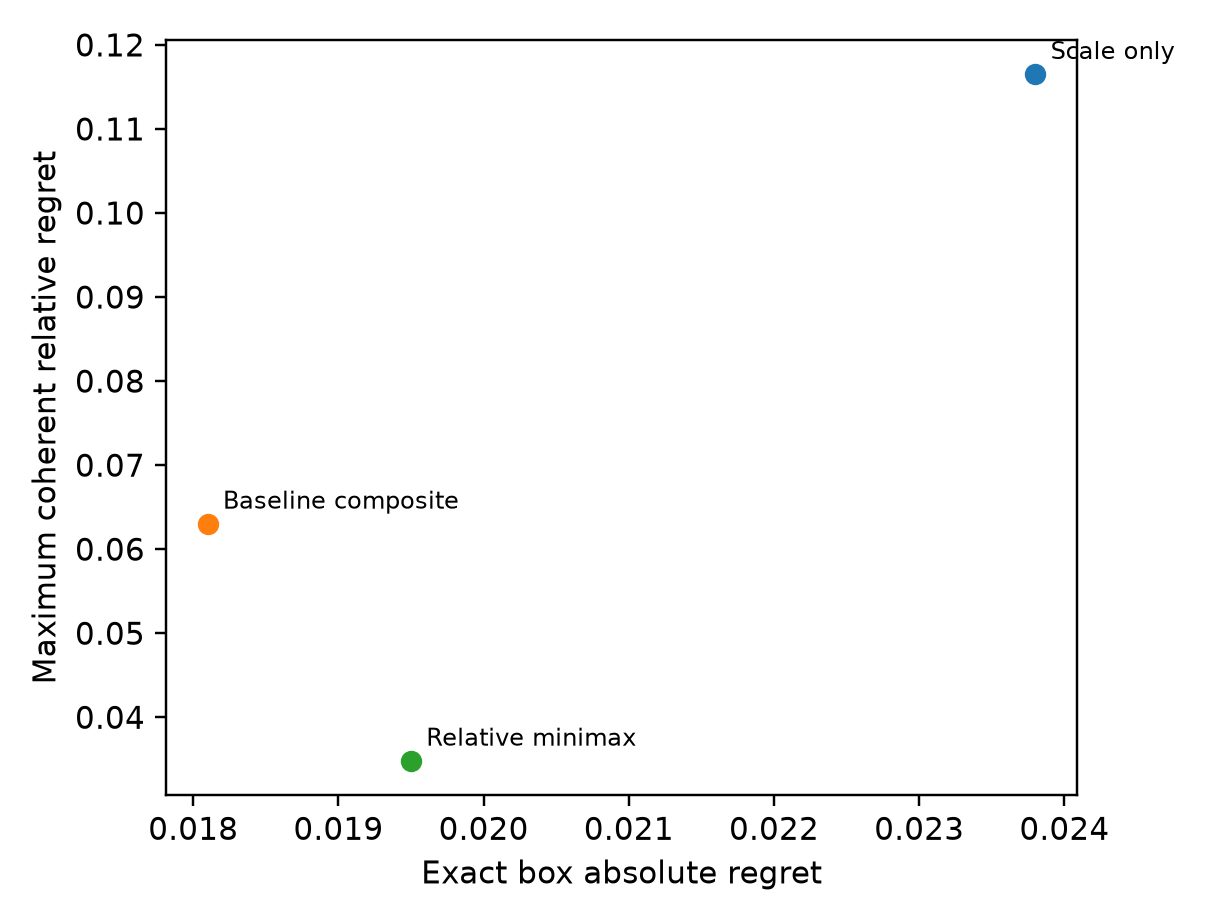
\includegraphics[width=.90\columnwidth]{figures/tradeoff.png}
\caption{Robustness trade-off at $k=25$. Lower values are preferred on both axes. Consensus-Frequency lies close to relative minimax but has higher coherent worst-case regret; the baseline composite retains the smallest independent-box regret.}
\label{fig:trade}
\end{figure}

\section{Practical Interpretation and Limits}
The results show why occupational AI prioritization should not be treated as one fixed ranking. Some occupations remain priority candidates across all 18 admitted constructions, while 23 additional occupations enter or leave the Top-25 depending on measurement design. For analysts or institutions that require one fixed screening list, the relative-minimax solution is a defensible compromise because it maximizes the worst retained share of scenario-optimal priority mass across the declared designs. The 24/25 overlap with the simple Consensus-Frequency benchmark indicates close agreement between the two lists, while the lower worst-case regret identifies the specific protection provided by the minimax criterion.

The uncertainty family is finite and reflects admitted measurement choices rather than a probability law. Stochastic acceptability analysis and budgeted-uncertainty optimization address different decision questions \cite{lahdelma1998,goerigk2025}. The present list is intended for screening and further assessment. It does not estimate AI-caused displacement, worker movement, training eligibility, transition capacity, or program success. Employment is a scale variable rather than a welfare weight.

\section{Conclusion}
Across 661 U.S. occupations, AI-exposure disagreement materially affects who enters a Top-25 priority list. Yet the disagreement is structured: 14 occupations are stable across all coherent designs and 37 form the coherent candidate envelope. Exact interval ranks distinguish guaranteed from merely possible membership, while coherent minimax supplies one fixed list when a decision must be made. Relative minimax raises worst-scenario capture from 93.70\% to 96.52\% compared with the baseline composite and retains 24/25 occupations from the Consensus-Frequency benchmark, without claiming universal robustness. Exact breakpoint semantics prevent equality/tie conventions from being mistaken for new membership at a boundary. The contribution is therefore an applied occupational-screening result supported by exact optimization certificates, rather than an optimization method presented with a workforce example.

\medskip
\noindent\textbf{Data and Code Availability---} The data, code, scenario matrices, selected lists, and reproducibility materials supporting this study are publicly available in the project \href{https://github.com/shaikhamalkawi-ux/When-AI-Exposure-Rankings-Disagree-Robust-Top-k-Occupational-Selection-under-Uncertainty}{\textbf{GitHub}~\raisebox{0.15ex}{\scriptsize$\nearrow$}}.

\begin{thebibliography}{30}\footnotesize
\bibitem{yin2026} M. Yin, H. Vu, and C. Persico, ``How (un)Stable Are LLM Occupational Exposure Scores? Evidence from Multi-Model Replication,'' NBER Working Paper 35110, 2026, doi: 10.3386/w35110.
\bibitem{felten2021} E. W. Felten, M. Raj, and R. Seamans, ``Occupational, industry, and geographic exposure to artificial intelligence: A novel dataset and its potential uses,'' \emph{Strategic Management Journal}, vol. 42, no. 12, pp. 2195--2217, 2021, doi: 10.1002/smj.3286.
\bibitem{tomlinson2025} K. Tomlinson, S. Jaffe, W. Wang, S. Counts, and S. Suri, ``Working with AI: Measuring the Applicability of Generative AI to Occupations,'' arXiv:2507.07935, 2025, doi: 10.48550/arXiv.2507.07935.
\bibitem{bls2026} U.S. Bureau of Labor Statistics, \emph{Occupational Employment and Wage Statistics, May 2025 National Estimates}, 2026.
\bibitem{onet2026} U.S. Department of Labor, Employment and Training Administration, \emph{O*NET 30.3 Database}, May 2026 release.
\bibitem{oecd2008} OECD and Joint Research Centre, \emph{Handbook on Constructing Composite Indicators: Methodology and User Guide}. OECD Publishing, 2008, doi: 10.1787/9789264043466-en.
\bibitem{manski2003} C. F. Manski, \emph{Partial Identification of Probability Distributions}. New York, NY, USA: Springer, 2003.
\bibitem{greco2008} S. Greco, V. Mousseau, and R. S\l{}owi\'nski, ``Ordinal regression revisited: Multiple criteria ranking using a set of additive value functions,'' \emph{European Journal of Operational Research}, vol. 191, no. 2, pp. 416--436, 2008.
\bibitem{steegen2016} S. Steegen, F. Tuerlinckx, A. Gelman, and W. Vanpaemel, ``Increasing transparency through a multiverse analysis,'' \emph{Perspectives on Psychological Science}, vol. 11, no. 5, pp. 702--712, 2016.
\bibitem{simonsohn2020} U. Simonsohn, J. P. Simmons, and L. D. Nelson, ``Specification curve analysis,'' \emph{Nature Human Behaviour}, vol. 4, pp. 1208--1214, 2020.
\bibitem{soliman2009} M. A. Soliman and I. F. Ilyas, ``Ranking with uncertain scores,'' in \emph{Proc. IEEE ICDE}, 2009, pp. 317--328.
\bibitem{mouratidis2015} K. Mouratidis, J. Zhang, and H. Pang, ``Maximum rank query,'' \emph{Proceedings of the VLDB Endowment}, vol. 8, no. 12, pp. 1554--1565, 2015.
\bibitem{mouratidis2018} K. Mouratidis and B. Tang, ``Exact processing of uncertain top-k queries in multi-criteria settings,'' \emph{Proceedings of the VLDB Endowment}, vol. 11, no. 8, pp. 866--879, 2018.
\bibitem{bertsimas2003} D. Bertsimas and M. Sim, ``Robust discrete optimization and network flows,'' \emph{Mathematical Programming}, vol. 98, pp. 49--71, 2003, doi: 10.1007/s10107-003-0396-4.
\bibitem{bertsimas2004} D. Bertsimas and M. Sim, ``The price of robustness,'' \emph{Operations Research}, vol. 52, no. 1, pp. 35--53, 2004, doi: 10.1287/opre.1030.0065.
\bibitem{bertsimas2011} D. Bertsimas, D. B. Brown, and C. Caramanis, ``Theory and applications of robust optimization,'' \emph{SIAM Review}, vol. 53, no. 3, pp. 464--501, 2011, doi: 10.1137/080734510.
\bibitem{aissi2009} H. Aissi, C. Bazgan, and D. Vanderpooten, ``Min--max and min--max regret versions of combinatorial optimization problems: A survey,'' \emph{European Journal of Operational Research}, vol. 197, no. 2, pp. 427--438, 2009.
\bibitem{ide2016} J. Ide and A. Sch\"obel, ``Robustness for uncertain multi-objective optimization,'' \emph{OR Spectrum}, vol. 38, pp. 235--271, 2016.
\bibitem{roy2010} B. Roy, ``Robustness in operational research and decision aiding: A multi-faceted issue,'' \emph{European Journal of Operational Research}, vol. 200, no. 3, pp. 629--638, 2010.
\bibitem{averbakh2005} I. Averbakh, ``Computing and minimizing the relative regret in combinatorial optimization with interval data,'' \emph{Discrete Optimization}, vol. 2, no. 4, pp. 273--287, 2005.
\bibitem{kouvelis1997} P. Kouvelis and G. Yu, \emph{Robust Discrete Optimization and Its Applications}. Boston, MA, USA: Kluwer, 1997.
\bibitem{savage1951} L. J. Savage, ``The theory of statistical decision,'' \emph{Journal of the American Statistical Association}, vol. 46, no. 253, pp. 55--67, 1951.
\bibitem{conde2004} E. Conde, ``An improved algorithm for selecting $p$ items with uncertain returns,'' \emph{Mathematical Programming}, vol. 100, no. 2, pp. 345--353, 2004.
\bibitem{kasperski2008} A. Kasperski, \emph{Discrete Optimization with Interval Data: Minmax Regret and Fuzzy Approach}. Berlin, Germany: Springer, 2008.
\bibitem{kasperski2010} A. Kasperski and P. Zieli\'nski, ``Minmax regret approach and optimality evaluation in combinatorial optimization problems with interval and fuzzy weights,'' \emph{European Journal of Operational Research}, vol. 200, no. 3, pp. 680--687, 2010, doi: 10.1016/j.ejor.2009.01.044.
\bibitem{dubois2016} D. Dubois and H. Prade, ``Practical methods for constructing possibility distributions,'' \emph{International Journal of Intelligent Systems}, vol. 31, no. 3, pp. 215--239, 2016, doi: 10.1002/int.21782.
\bibitem{lahdelma1998} R. Lahdelma, J. Hokkanen, and P. Salminen, ``SMAA---stochastic multiobjective acceptability analysis,'' \emph{European Journal of Operational Research}, vol. 106, no. 1, pp. 137--143, 1998, doi: 10.1016/S0377-2217(97)00163-X.
\bibitem{goerigk2025} M. Goerigk and M. Khosravi, ``Robust combinatorial optimization problems under budgeted interdiction uncertainty,'' \emph{OR Spectrum}, vol. 47, pp. 255--285, 2025, doi: 10.1007/s00291-024-00772-0.
\end{thebibliography}
\end{document}
